\subsubsection{Kubuntu 16.04}

Am Host-PC muss bei den IPv4-Einstellungen die Methode "`Automatisch"' eingestellt sein. Wenn es sich um eine neue Verbindung handelt, ist dies bereits voreingestellt, eine Parametrierung kann dann entfallen. Ansonsten muss zur Konfiguration unter Linux (Kubuntu 16.04) zuerst der Dialog "`Netzwerkverbindungen"' ge�ffnet werden.\\ 
Dazu klickt man mit der rechten Maustaste auf das Netzwerksymbol in Infobereich rechts unten. Dann kann die Option "`Netzwerkverbindungen einrichten..."' ausgew�hlt werden.

\begin{figure}[ht]
  \centering
  
\includegraphics[scale=1.00]{images/OTG_NetzwerkverbindungenIcon.png}	
  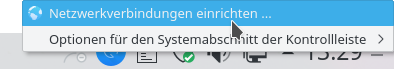
\includegraphics[scale=0.42]{images/OTG_NetzwerkverbindungenOpen.png}	
  %	\caption{}
  \label{OTG_LINUX_NetzwerkverbindungenApp}
\end{figure}


Nun k�nnte die neue "`Kabelnetzwerkverbindung"' umbenannt werden, z.~B. in Raspberry Pi Zero. Erkennen kann man das Netzwerk an der Mac-Adresse, die man bei "`g\_ether.host\_addr"' angegeben hat (z.~B. 00:01:02:03:04:05).  


\begin{figure}[ht]
  \centering
  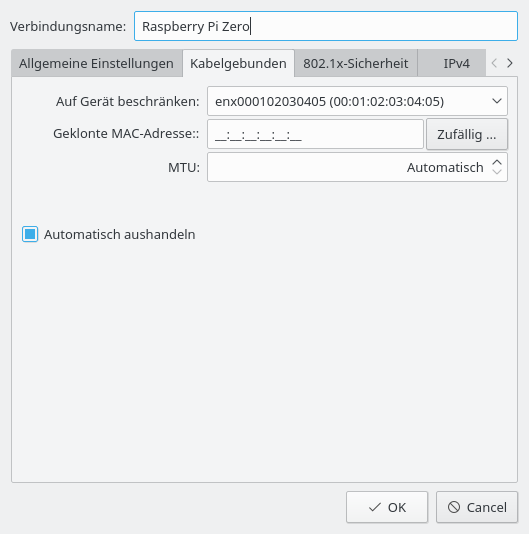
\includegraphics[scale=0.42]{images/OTG_Pi_Verbindungsname.png}
	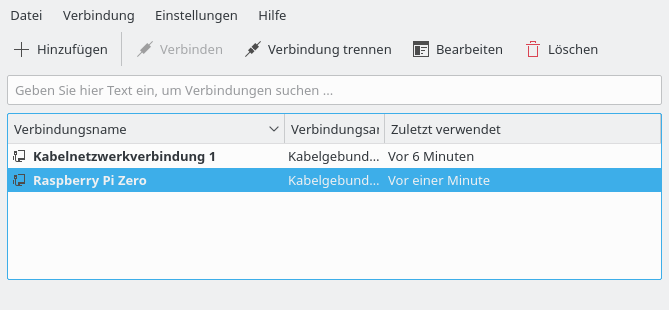
\includegraphics[scale=0.42]{images/OTG_Netzwerkverbindungen.png}
%	\caption{}
  \label{OTG_LINUX_Netzwerkverbindungen}
\end{figure}


Nun kann bei den IPv4-Einstellungen die Methode "`Automatisch"' eingestellt werden.

%\begin{figure}[ht]
%  \centering
%  \includegraphics[scale=0.42]{images/OTG_NetzwerkverbindungenAutomatisch.png}
%	\caption{}
%  \label{OTG_LINUX_Netzwerkverbindungen}
%\end{figure}
